
\documentclass{standalone}

\usepackage{tikz}
\usetikzlibrary{shapes}

\begin{document}

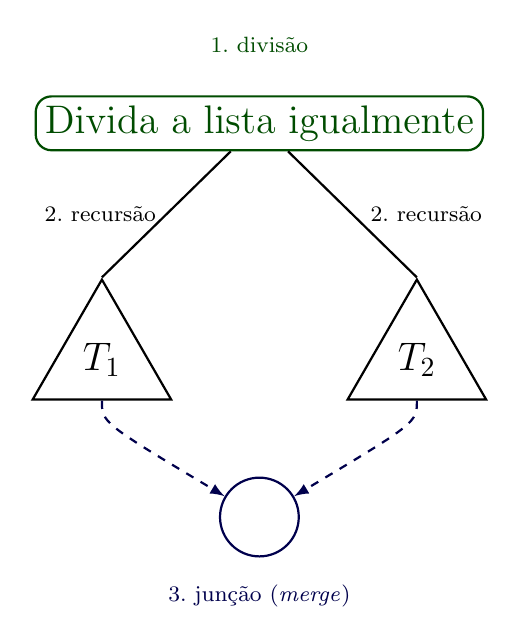
\begin{tikzpicture}
\def\D{2cm}
\def\dd{0}
\colorlet{divide color}{green!30!black}
\colorlet{merge color}{blue!30!black}
\tikzset{
  scale=.7,
  every node/.style={font=\Large},
  every path/.style={thick,draw},
  divide/.style={divide color,rounded corners=2mm,thick,draw},
  conquer/.style={conquer color,rounded corners=2mm,thick,draw},
  merge path/.style={->,>=latex,merge color,dashed,thick,draw},
  recursion/.style={regular polygon, regular polygon sides=3,draw},
  merge/.style={merge color,minimum width=\D/2,circle,draw}
}

%INIT
\node[divide] (LIST) {Divida a lista igualmente};
\node[divide color] [above of=LIST] {\footnotesize 1.~divis\~ao};

%RECURSION - COMPUTATION
\node[recursion] (T1) [below of=LIST,yshift=-\D,xshift=-\D] {$T_1$};
\node[recursion] (T2) [below of=LIST,yshift=-\D,xshift=\D] {$T_2$};

%MERGE - HALT
\node[merge] (MERGE) [below of=LIST, yshift=-2*\D]{};
\node[merge color] [below of=MERGE] {\footnotesize 3.~jun\c{c}\~ao ({\it merge\/})};

%PATHS
\path (LIST) -- node[left] {\footnotesize\ 2.~recurs\~ao} (T1.north);
\path (LIST) -- node[right] {\footnotesize\ 2.~recurs\~ao} (T2.north);
%%merge
\path[merge path] (T1.south) .. controls  +(down:4mm) .. (MERGE);
\path[merge path] (T2.south) .. controls  +(down:4mm) .. (MERGE);

\end{tikzpicture}

\end{document}

